\section{Caratteristiche generali del dializzatore}

Durante il trattamento dialitico, il dializzatore è il luogo in cui avviene il trasporto di massa sia \textit{dal} paziente (es. potassio e cataboliti) che \textit{verso} il paziente (es. bicarbonato). Qui avviene anche il trasporto di acqua dal paziente al dialisato. Questi due tipi di trasporto sono regolati dalla \textit{differenza di concentrazione} nel caso dei soluti, e dalla \textit{differenza di pressione} nel caso dell'acqua.

In un dializzatore è possibile regolare, in base alle circostanze, sia la portata di sangue in ingresso che la portata del dialisato.
Poiché dialisato e filtrato (cioè l'acqua estratta dal sangue durante il passaggio nel dializzatore) sono fluidi omogenei, la misura dei loro flussi è pari alla loro portata volumetrica. Il sangue, invece, è un fluido eterogeneo contenente una parte corpuscolata, gli eritrociti, e una parte in sospensione acquosa, le proteine; pertanto la portata volumetrica di sangue è sempre superiore alla portata di acqua che effettivamente esso contiene, ed è la sola portata di acqua che bisogna considerare nei calcoli dei processi di trasporto. Tale portata di acqua si calcola nel seguente modo: 
%$$\frac{acqua}{secondo}=\frac{sangue}{secondo}\cdot\frac{plasma}{sangue}\cdot\frac{acqua}{plasma}$$
%cioè,
\begin{equation}
	Q_b = Q_B\biggl(1-\frac{Hct}{100}\biggr)F_p \label{Qeff}
\end{equation}
dove $Q_b$ è la portata effettiva di acqua ($L/sec$), $Q_B$ è la portata del prelievo ematico, $(1-Hct/100)$ è la frazione di plasma nel sangue e $Fp$ è la frazione di acqua nel plasma, quest'ultima calcolata con la formula di Colton et al. \cite{colton}:
\begin{equation}
	F_p = 1-0.0107\cdot Tp
	\label{eq:colton}
\end{equation}
in cui $T_p$ è la concentrazione totale delle proteine plasmatiche, espressa in $gr/dL$.\\
In questa trattazione si fa l'ipotesi che la membrana dell'eritrocita sia impermeabile e all'acqua e ai soluti\footnote{in realtà, anche i globuli rossi contengono acqua e soluti che partecipano, seppur in minima parte, agli scambi diffusivi e convettivi. Per approfondimenti si veda Sargent et al. \cite{sargent}}.

In \figurename\ref{dialyzer} è schematizzato un dializzatore, con le portate e concentrazioni dei fluidi in ingresso e in uscita.
\begin{figure}[htb]
	\centering
		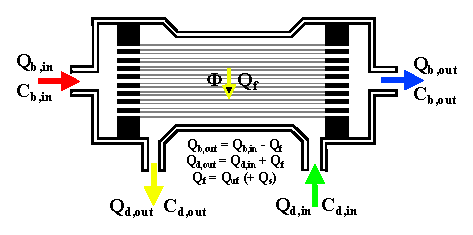
\includegraphics[width=0.6\textwidth]{immagini/dialyzer.eps}
		\caption{Rappresentazione schematica dei flussi e delle concentrazioni per un dializzatore operante con flussi in contro-corrente. La grandezza $Q_s$ è opzionale e dipende dalla modalità di dialisi.}\label{dialyzer}
\end{figure}

Indipendentemente dalla modalità di dialisi (emodialisi o emodiafiltrazione), il bilancio ingresso-uscita riguardo al compartimento \textit{sangue} è dato dal seguente sistema:
\begin{equation}\label{bilancio}
	\begin{cases}
	Q_{b_{out}}C_{b_{out}} =Q_{b_{in}}C_{b_{in}}-\Phi & \text{  bilancio di massa}\\
	Q_{b_{out}} =Q_{b_{in}}-Q_f & \text{  bilancio di volume}\\
	\end{cases}
\end{equation}
in cui con $Q_f$ si è indicata la portata di acqua filtrata dal dializzatore\footnote{nell'emodialisi $Q_f$ è pari all'ultrafiltrazione $Q_{uf}$, cioè alla quantità di liquido da togliere al paziente nell'unità di tempo affinché raggiunga, a fine dialisi, il peso desiderato. Nell'emodiafiltrazione, $Q_f$ è dato da $Q_{uf}$ sommata alla portata $Q_s$ del fluido di diluizione.}.
La quantità $\Phi$ di soluto eliminata nell'unità di tempo dal dializzatore è quindi:
\begin{equation}\label{general1}
\Phi = Q_{b_{in}} (C_{b_{in}} - C_{b_{out}}) + Q_f C_{b_{out}}
\end{equation}
La \textit{Dialisance} è un parametro unico per ogni coppia dializzatore-soluto, ed è definita come la ``variazione di soluto nel sangue per unità di differenza di concentrazione (\textit{utile} alla diffusione) fra compartimento sangue e dialisato, in assenza di ultrafiltrazione'', ovvero:
\begin{equation*}
	D := \frac{Q_{b_{in}}(C_{b_{in}}-C_{b_{out}})}{\alpha C_{b_{in}} - C_{d_{in}}}
\end{equation*}
Il termine \textit{utile} si riferisce all'effetto \textit{Donnan} (\textsection\ref{sec:donnan}), codificato dal coefficiente $\alpha$; $C_{d_{in}}$ è la concentrazione in ingresso, del soluto disciolto nel liquido dializzante, d'ora in poi indicata con $C_d$. Alla luce di ciò si può riscrivere la (\ref{general1}) come:
\begin{equation}\label{general2}
	\Phi = D \biggl(\alpha C_{b_{in}} - C_d\biggr) + Q_f C_{b_{out}}
\end{equation}
L'equazione~(\ref{general2}) è valida in generale per qualsiasi dializzatore, indipendentemente dalla modalità di dialisi. L'obiettivo è però quello di cercare una formula per $\Phi$ che sia dipendente dai soli parametri di portata, dialisance e dalle sole concentrazioni in ingresso, perché più facilmente determinabili nella pratica clinica. Lo scopo dei prossimi due paragrafi è appunto quello di ricavare un'espressione per l'emodialisi e per l'emo\-dia\-fil\-tra\-zio\-ne che abbia tali caratteristiche. Per snellire la scrittura si userà il pedice \textit{i} al posto del pedice \textit{$b_{in}$} per riferirsi alla portata e alla concentrazione della soluzione plasmatica in ingresso al dializzatore.

\section{Caratteristiche del dializzatore per HD}
Nel caso dell'emodialisi il flusso di massa $\Phi$ estratto dal dializzatore è prevalentemente di tipo diffusivo, cioè:
\begin{equation}\label{phihd}
	\Phi=\Phi_d
\end{equation}
in cui il pedice \textit{d} indica appunto la natura diffusiva dello scambio. Sostituendo le equazioni (\ref{general2}) e (\ref{phihd}) nel sistema (\ref{bilancio}) e ricavando $\Phi_d$, si ottiene:
\begin{equation}\label{phidemo}
	\Phi_d = D (\alpha C_i - C_d)\biggl(1-\frac{Q_f}{Q_i}\biggr) + Q_f C_i
\end{equation}
In questa equazione, il termine di trasporto convettivo $Q_f C_i$ non deve essere considerato come un effettivo meccanismo \textit{fisico} di trasporto perché, nell'emodialisi, il passaggio di soluto non avviene per convezione. Si tratta invece di un termine di trasporto \textit{matematico} di correzione, che tiene conto dell'influenza positiva dell'ultrafiltrazione sull'aumento del gradiente di concentrazione a cavallo della membrana e, quindi, sull'aumento della diffusione attraverso di essa \cite{sargent}.

Viene definita \textit{frazione di filtrazione} il rapporto fra l'acqua filtrata e l'acqua in ingresso al dializzatore:
$$FF := \frac{Q_f}{Q_i}$$
La frazione di filtrazione, a meno che non vengano filtrati anche globuli rossi e proteine, assume valori fra zero e uno. Si può dunque riscrivere la (\ref{phidemo}) nel modo seguente:
\begin{equation}\label{phidFF}
	\Phi_d = (1-FF)\cdot D(\alpha C_i - C_d) + FF\cdot Q_i C_i
\end{equation}
Si noti ora che il flusso $\Phi_d$ è composto da due termini: il primo diffusivo, proporzionale a $(1-FF)$, cioè alla frazione di acqua non filtrata dal dializzatore; il secondo di correzione, proporzionale alla frazione di acqua che fitra nel compartimento del dialisato.
Facendo un calcolo esemplificativo per una seduta emodialitica \textit{standard}, in cui si imposta un flusso di filtrazione pari a $1$~$L/h$ e un flusso di fistola di $300$~$mL/min$, si ottiene:
$$ FF < 0.06 $$
$$ (1-FF) > 0.94 $$
e cioè che nell'emodialisi, la correzione da aggiungere al fenomeno di trasporto principale ha un basso indice di importanza.

\section{Caratteristiche del dializzatore per HDF}\label{sec:HDF}
In letteratura è più volte affermato che nell'emodiafiltrazione, a causa di un'interazione di tipo competitiva fra convezione e diffusione, il trasporto combinato non è dato dalla somma dei singoli fenomeni, ma è più complesso \cite{hoenich,canaud}. Questi tipi di flusso sono quindi dipendenti l'uno dall'altro, e dipendono anche da $Q_f$, cioè:
\begin{equation}\label{phidf}
	\Phi(Q_f) = \Phi_d(Q_f,\Phi_t) + \Phi_t(Q_f,\Phi_d)
\end{equation}
Si può ipotizzare che, in presenza simultanea delle due modalità di trasporto, e a parità delle altre condizioni fluidodinamiche, la capacità di purificazione dell'HDF sia maggiore delle singole \textit{performance} di emodialisi ed emofiltrazione. Si può quindi ipotizzare che almeno in prima approssimazione i fenomeni di trasporto convettivo e diffusivo siano additivi. Se così non fosse, nessun medico avrebbe finora scelto l'HDF come tecnica dialitica per i propri pazienti. Un'altra ipotesi è che all'aumentare della portata di filtrazione, lo strato proteico che si deposita all'interno della membrana del dializzatore renda meno efficiente lo scambio di soluti \cite{colton}. Con queste considerazioni, la più semplice funzione per $\Phi$ è di tipo quadratica\footnote{la funzione più semplice non può essere di tipo lineare perché, per i motivi spiegati, in HDF non vale il principio di \textit{sovrapposizione degli effetti}.}, in particolare una parabola con la concavità verso il basso (\figurename~\ref{fig:PHI}); una funzione di questo tipo, infatti, descrive bene sia l'additività dei due fenomeni di trasporto a bassi regimi di filtrazione che il calo di prestazioni a frazioni di filtrazione più elevate.
\begin{figure}[htbp]
	\centering
		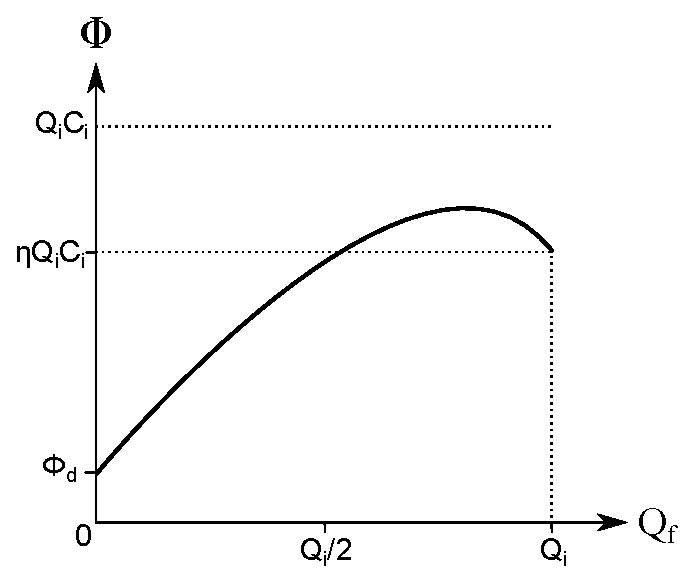
\includegraphics[width=0.70\textwidth]{immagini/hp_hdf.eps}
	\caption{ipotetica funzione per $\Phi(Q_f)$}
	\label{fig:PHI}
\end{figure}

La portata di filtrazione $Q_f$ varia da un minimo di zero a un massimo di $Q_i$ (non è possibile infatti estrarre dal dializzatore più di quanto non vi entri). La funzione che si sta cercando ha quindi la forma:
\begin{equation}\label{phi}
		\Phi(Q_f) = a\cdot Q_f^2 + b\cdot Q_f + c  \text{,\qquad$Q_f$ $\in[0-Q_i]$}
\end{equation}\\
I coefficienti $a$, $b$ e $c$ possono essere ricavati imponendo le seguenti condizioni al contorno:
\begin{subequations}\label{cc}
	\begin{align}
		&\Phi(0)=\Phi_d\label{cc0}\\
		&\Phi(Q_i)=\eta \cdot Q_i C_i\label{cc1}\\
		&\frac{d\Phi}{dQ_f}\Biggr\rvert_{Q_f=0}=\frac{\partial\Phi_d}{\partial Q_f} + \frac{\partial\Phi_t}{\partial Q_f}\label{ccd}
	\end{align}
\end{subequations}
La condizione (\ref{cc0}) indica che in assenza di filtrazione il flusso $\Phi$ è puramente diffusivo e pari a (\ref{phidemo}); la condizione (\ref{cc1}) indica che quando $Q_f$ è massimo, il soluto estratto dal compartimento ematico è pari al flusso di soluto in ingresso al dializzatore, corretto dal coefficiente $\eta<1$, per tener conto della limitazione introdotta dallo strato proteico; la condizione (\ref{ccd}) è stata invece ricavata col seguente ragionamento.
Considerando la (\ref{phidf}) e calcolandone il differenziale si ottiene:
\begin{equation}\label{diff}
	d\Phi = \frac{\partial \Phi_d}{\partial Q_f} \cdot dQ_f + \frac{\partial \Phi_d}{\partial \Phi_t} \cdot d\Phi_t
					+ \frac{\partial \Phi_t}{\partial Q_f} \cdot dQ_f + \frac{\partial \Phi_t}{\partial \Phi_d} \cdot d\Phi_d
\end{equation}
È possibile ipotizzare che quando $Q_f\approxeq 0$, i flussi $\Phi_d$ e $\Phi_t$ siano indipendenti l'uno dall'altro; infatti, in questa condizione, il flusso trasportato per convezione è anche esso trascurabile, e non influenza il gradiente di concentrazione a cavallo della membrana utile alla diffusione; allo stesso modo, un eventuale passaggio di soluto per diffusione non influenza il flusso convettivo (\ref{phit}) poiché il soluto trasportato, essendo pari al valor medio $(C_i+C_D)/2$ (\textsection\ref{sec:convettivo}), resta invariato, in quanto una diminuzione di $C_i$ è compensata da un aumento di pari entità di $C_D$.
Per le considerazioni fatte ora, i termini ~$\partial \Phi_d/\partial \Phi_t$ e ~$\partial \Phi_t/\partial \Phi_d$ nella (\ref{diff}) possono considerarsi nulli. Quindi, con l'ipotesi di $Q_f$ trascurabile, la derivata del flusso totale di soluto rispetto alla portata di filtrazione è:\\
\begin{equation}\label{diff1}
	\frac{d\Phi}{dQ_f}\Biggr\rvert_{Q_f=0} = \frac{\partial \Phi_d}{\partial Q_f} + \frac{\partial \Phi_t}{\partial Q_f}
\end{equation}
che corrisponde alla terza condizione al contorno, necessaria per identificare univocamente la funzione parabolica.
Le funzioni delle quali interessa calcolare le derivate parziali da inserire nella (\ref{diff1}) sono:
\begin{subequations}\label{phidt}
		\begin{align}
			&\Phi_d = D (\alpha C_i - C_D)\biggl(1-\frac{Q_f}{Q_i}\biggr) + Q_f C_i\\
			&\Phi_t = Q_f \varepsilon C_M\label{phit}
		\end{align}
	\end{subequations}
dove l'equazione per $\Phi_d$ è la stessa della (\ref{phidemo}), e l'equazione per $\Phi_t$ è analoga alla (\ref{phiT}). Le derivate parziali, calcolate rispetto al flusso di filtrazione, sono:
\begin{subequations}\label{derphidt}
		\begin{align}
			&\frac{d\Phi_d}{dQ_f} = C_i -\frac{D}{Q_i}(\alpha C_i - C_d)\\
			&\frac{d\Phi_t}{dQ_f} = \varepsilon C_M
		\end{align}
	\end{subequations}
Le (\ref{derphidt}) sostituite nella (\ref{diff1}) esplicitano la condizione al contorno (\ref{ccd}).\\
Risolvendo ora la (\ref{phi}) con le condizioni al contorno (\ref{cc}) si ottengono i seguenti valori per i coefficienti $a$, $b$ e $c$:\\
\begin{align*}
	a& = -\frac{1}{Q_i}\cdot \biggl[(1-\eta)C_i + \varepsilon C_M\biggr]\\
	b& = C_i - \frac{1}{Q_i}D(\alpha C_i - C_d)+ \varepsilon C_M\\
	c& = D(\alpha C_i - C_d)
\end{align*}
La formula per il flusso complessivo $\Phi$ in presenza contemporanea di dialisi ed emofiltrazione è pertanto:
\begin{equation}\label{phihdf}
	\begin{split}
	 \Phi_{hdf}& = D(\alpha C_i - C_d)\biggl(1-\frac{Q_f}{Q_i}\biggr)+Q_f C_i + Q_f \varepsilon C_M\biggl(1-\frac{Q_f}{Q_i}\biggr) - (1-\eta)\frac{Q_f^2}{Q_i}C_i\\
		                & = (1-FF)\cdot \biggl[D(\alpha C_i - C_d)+\Phi_t \biggr] + FF\cdot \biggl[Q_i-(1-\eta)Q_f\biggr] C_i
	\end{split}
\end{equation}
Il flusso $\Phi_{hdf}$ è composto da due termini: il primo, somma di diffusione e convezione, proporzionale alla frazione di acqua non filtrata dal dializzatore; il secondo di correzione, proporzionale alla frazione di filtrazione.
Gli algoritmi interni della macchina dializzatrice fanno sì che, sia in pre- che in post-diluizione, la frazione di filtrazione sia pari a circa $0,5$. Il termine correttivo, a differenza del caso dell'emodialisi, ha quindi un peso molto importante nella determinazione della performance del dializzatore. Il coefficiente $\eta$ dovrà essere identificato per ogni seduta e per ogni soluto in quanto dipenderà dalla concentrazione proteica, variabile ad ogni seduta, e dall'interazione dello strato proteico coi diversi soluti.

A supporto del risultato teorico appena esposto, si mostrano i risultati sperimentali (\figurename\ref{pedr2}) ottenuti da Pedrini et al. \cite{pedrini2}.
\begin{figure}[htb]
	\centering
	\subfigure[]%
	{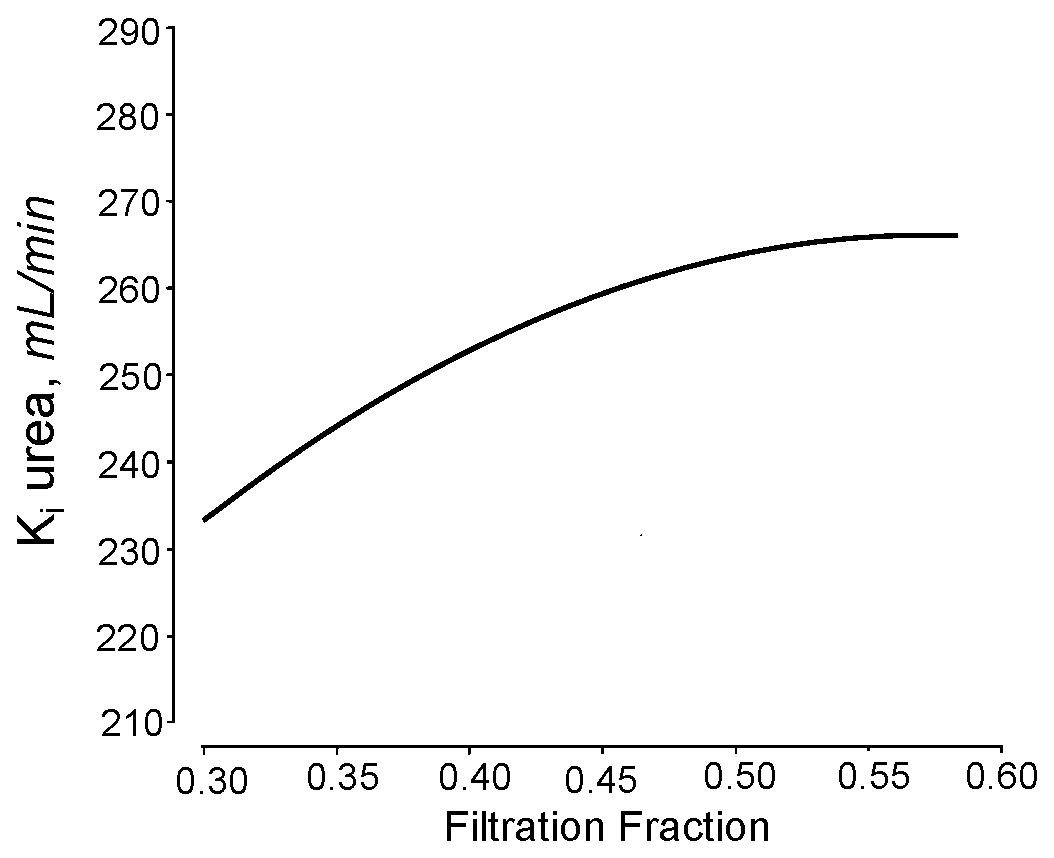
\includegraphics[width=0.30\textwidth]{immagini/pedrini2A.eps}}\quad
	\subfigure[]%
	{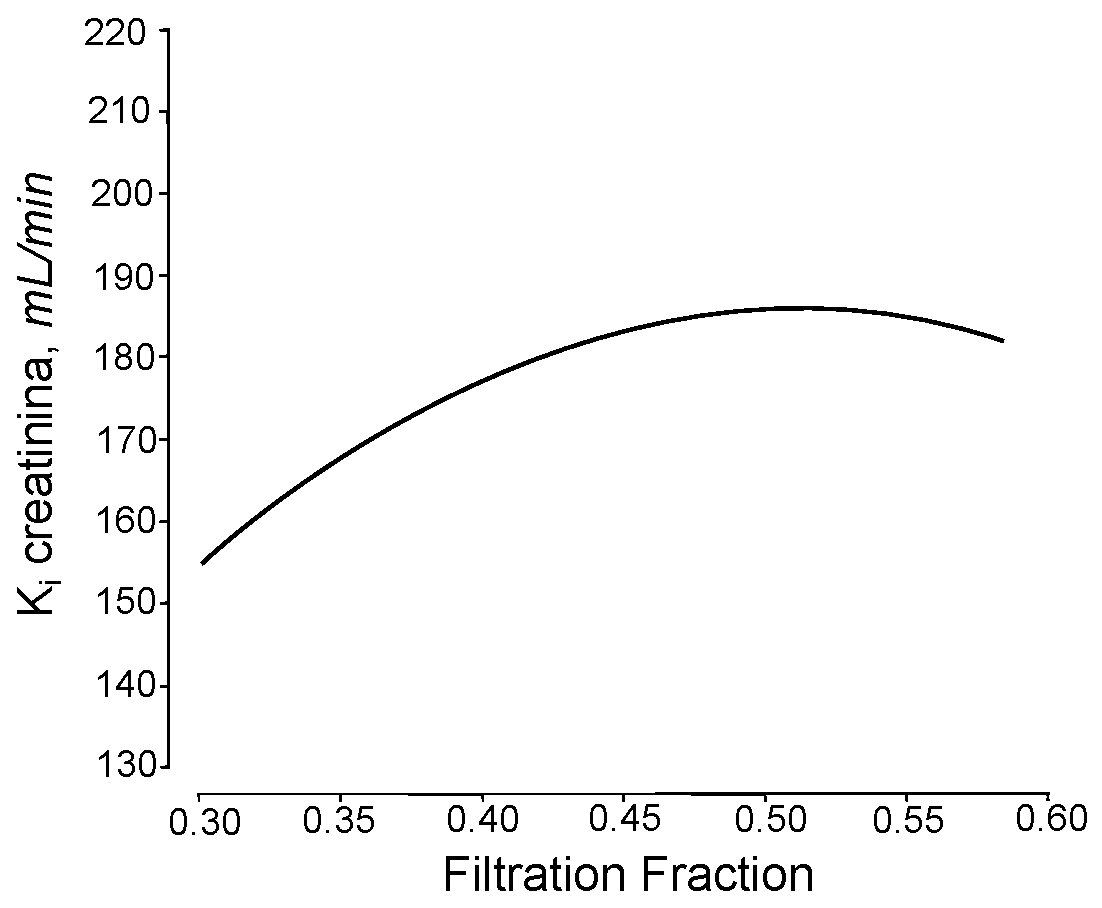
\includegraphics[width=0.30\textwidth]{immagini/pedrini2B.eps}}\quad
	\subfigure[]%
	{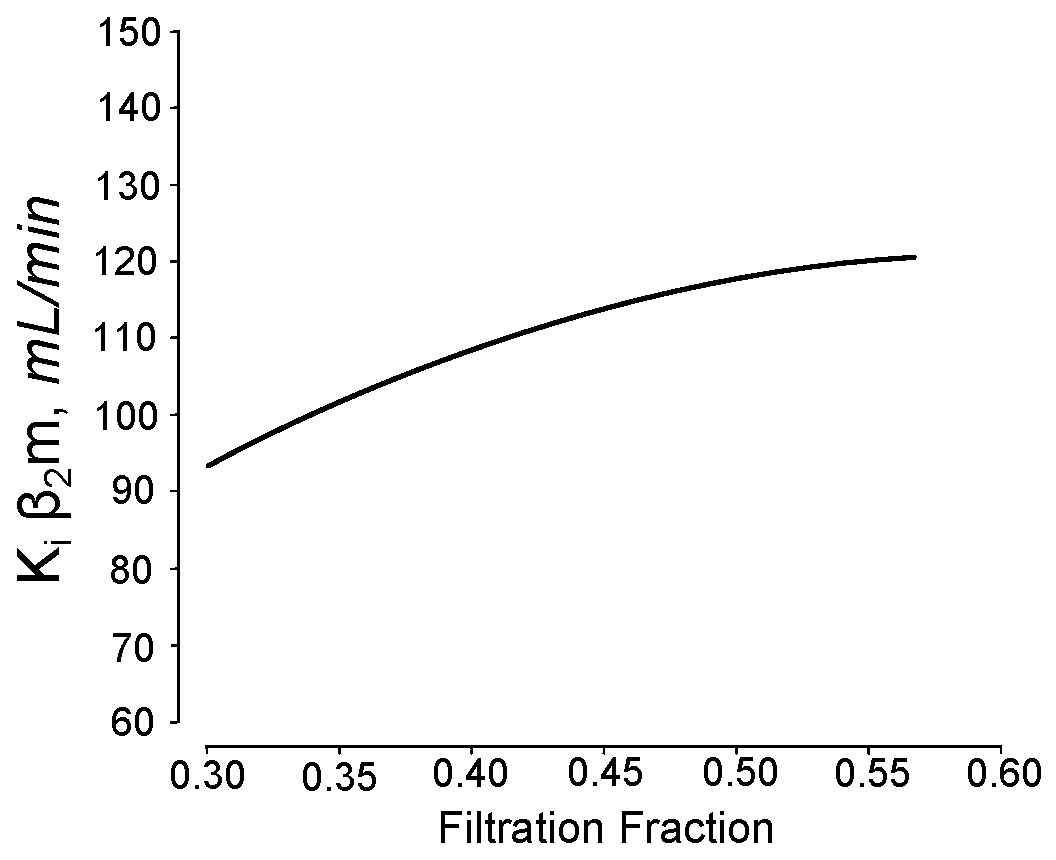
\includegraphics[width=0.30\textwidth]{immagini/pedrini2C.eps}}
		\caption{Interpolazione polinomiale del secondo ordine dei dati relativi alle \textit{clearance} ($K_i$) di (a) urea, (b) creatinina, e (c) $\beta_2m$, \textit{vs} $FF$.}\label{pedr2}
\end{figure}
Le \textit{clearance} dei tre soluti presentano un andamento parabolico con concavità verso il basso; in più possiamo considerare la clearance e il termine $\Phi$, ricavato in questo paragrafo, linearmente dipendenti (per l'omogeneità delle unità di misura). Per questi motivi i risultati di \figurename\ref{pedr2} sembrano non smentire la teoria fin qui sviluppata.
